\begin{frame}[noframenumbering]{Nonlinear Laplace: solver settings}
	\begin{itemize}
		\item $300\times 300$ elements per subdomain
		\item Averaging recombination
		\item Relative tolerance outer Newton: $10^{-4}$
		\item GMRES tolerance: $10^{-6}$
		\item Relative tolerance inner Newton: $10^{-5}$
		\item Absolute tolerance inner Newton: $10^{-11}$
		\item RGDSW coarse space
		\item Zero initial value
	\end{itemize}
\end{frame}

\begin{frame}[noframenumbering]{Neo-Hooke: Solver settings}
	\begin{columns}
		\begin{column}{0.55\textwidth}
			General settings:
			\vspace{7pt}
			\begin{itemize}
				\item Outer Newton rel. tol.  = $10^{-4}$
				\item Outer Newton max. iters. = $10$
				\item GMRES rel. tol. = $10^{-6}$
				\item GMRES max. its. = $100$
				\item GMRES max. restarts = $20$
				\item Recombination mode: averaging
        % Note: overlap used here is the dual graph overlap. Actual overlap used for NKS = 5 to correspond to similar physicial overlap
				\item Coarse space: MsFEM elasticity with overlap = $5$
			\end{itemize}
		\end{column}%
		\begin{column}{0.45\textwidth}
			Nonlinear Schwarz specific settings:
			\vspace{7pt}
			\begin{itemize}
				\item Inner Newton rel. tol. = $10^{-5}$
				\item Inner Newton abs. tol. = $10^{-9}$
				\item Inner Newton max. iters. = $15$
			\end{itemize}
		\end{column}
	\end{columns}
\end{frame}

\begin{frame}[noframenumbering]{LDC: solver settings}
	\begin{columns}
		\begin{column}{0.55\textwidth}
			General settings:
			\vspace{7pt}
			\begin{itemize}
				\item Subdomain size: $150\times 150$ elements
				\item Outer Newton rel. tol.  = \num{e-6}
				\item Outer Newton abs. tol.  = \num{e-6}
        \item Backtracking line-search
				\item GMRES rel. tol. = \num{e-4}
				\item GMRES max. its. = $1000$
				\item Krylov subspace dim. = $500$
				\item Recombination mode: averaging
				\item Coarse space: MsFEM with overlap = $5$
			\end{itemize}
		\end{column}%
		\begin{column}{0.45\textwidth}
			Nonlinear Schwarz specific settings:
			\vspace{7pt}
			\begin{itemize}
				\item Inner Newton rel. tol. = \num{e-3}
				\item Inner Newton abs. tol. = \num{e-14}
				\item Inner Newton max. iters. = $50$
				\item H1 variant
			\end{itemize}
		\end{column}
	\end{columns}
\end{frame}



\begin{frame}[noframenumbering]{Motivation: linear vs nonlinear preconditioning}
	Discretized nonlinear partial differential equation: $F(u) = 0$
	\begin{columns}
		\begin{column}{0.5\textwidth}
			\vspace*{-4mm}
			\begin{block}{\normalsize Linear preconditioner}
				\begin{enumerate}
					\item Linearize:
					      \begin{equation*}
						      DF(u^k)\delta^{k+1} = F(u^k)
					      \end{equation*}
					\item Improve linear solver performance with Schwarz preconditioner:
					      \begin{equation*}
						      \mathcal{M}_{OS}^{-1}DF(u^k)\delta^{k+1} = \mathcal{M}_{OS}^{-1}F(u^k)
					      \end{equation*}
				\end{enumerate}
				\vspace*{4mm}
				Goal:
				\begin{itemize}
					\item $\kappa(\mathcal{M}_{OS}^{-1}DF(u^k)) \approx 1$
				\end{itemize}
			\end{block}
		\end{column}
		\begin{column}{0.5\textwidth}
			\vspace*{-4mm}
			\begin{block}{\normalsize Nonlinear preconditioner}
				\begin{enumerate}
					\item Reformulate the original nonlinear problem based on local nonlinear corrections
					      \begin{equation}
						      \mathcal{F}(u) = G(F(u)) = 0
					      \end{equation}
					\item Linearize $\mathcal{F}(u) = 0$ and solve iterativily
				\end{enumerate}
				Goal:
				\begin{itemize}
					\item $\mathcal{F}(u)$ more linear than $F(u)$
					\item $\mathcal{F}(u^*) = 0 \iff F(u^*) = 0$
				\end{itemize}
			\end{block}
		\end{column}
	\end{columns}

\end{frame}

\begin{frame}[noframenumbering]{One-level nonlinear Schwarz}
	\note{This requires two levels of Newton's method. Seems to be less efficient at first glance. The advantage of this method becomes apparent when solving problems with local regions of highly nonlinear behavior e.g. laminar flow with localized turbulence\\}
	\note{The algorithm shows how this method is essentially the same as applying Newton directly, but to the function $\mathcal{F}$ instead of $F$.\\}
	\note{Constructin $A$ requires inversion of all the local matrices. The result of this is that the linear system is already preconditioned. Note that the preconditioner can not be changed on the fly. It results directly from the nonlinear problem}
	\begin{columns}
		\begin{column}{0.53\textwidth}
			\begin{algorithm}[H]
				\small
				\begin{algorithmic}[1]
					\State $k\gets0$
					\State \textbf{Init.} $u^k$
					\State \textbf{Eval.} $F(u^k)$
					\While{stop. cond. false}
					\State \textbf{Eval.} $\mathcal{F}_1(u^k)$
					\State \textbf{Eval.} $D\mathcal{F}_1(u^k)$
					\State \textbf{Solve} (e.g. GMRES) $D\mathcal{F}_1(u^k)\delta^k = \mathcal{F}_1(u^k)$
					\State \textbf{Update} $u^{k+1} = u^k - \delta^k$
					\State $k\gets k+1$
					\State \textbf{Eval.} $F(u^k)$
					\EndWhile
				\end{algorithmic}
				\caption*{\small Nonlinear Schwarz}
			\end{algorithm}
		\end{column}
		\begin{column}{0.47\textwidth}
			\begin{algorithm}[H]
				\small
				\begin{algorithmic}[1]
					\State $k \gets 0$
					\State \textbf{Init.} $g_i^k$
					\State \textbf{Eval.} $F_i^k\coloneqq R_iF(u-P_ig_i^k)$
					\While{stop. cond. false}
					\State \textbf{Eval.} $DF_i^k= R_iDF(u-P_ig_i^k)P_i$
					\State \textbf{Solve} (direct) $DF_i^k\delta^k = F_i^k$
					\State \textbf{Update} $g_i^{k+1} = g_i^k + \delta^k$
					\State $k\gets k+1$
					\State \textbf{Eval.} $F_i^k\coloneqq R_iF(u-P_ig_i^k)$
					\EndWhile
					\State $g_i\gets g_i^k$
				\end{algorithmic}
				\caption*{\small Evaluation of $g_i\coloneqq T_i(u)$}
			\end{algorithm}
		\end{column}
	\end{columns}
\end{frame}

\begin{frame}[noframenumbering]{Adding a coarse level \footnote{\tiny Toselli, Widlund (2005)}}

	{\Large Linear Schwarz preconditioners}
	\vspace*{4mm}
	\begin{columns}
		\begin{column}{0.5\textwidth}
			{\bf One-level Schwarz preconditioner}
			\begin{equation*}
				\mathcal{M}^{-1}_{OS-1}=\sum_{i=1}^{N}P_i(R_iAP_i)^{-1}R_i
			\end{equation*}
			\begin{block}{\normalsize Condition number estimate:}
				\begin{equation*}
					\kappa(\mathcal{M}^{-1}_{OS-1}A)\leq C(1+\frac{1}{H\delta})
				\end{equation*}
			\end{block}
		\end{column}
		\begin{column}{0.5\textwidth}
			{\bf Two-level Schwarz preconditioner}
			\vspace*{3mm}
			\begin{equation*}
				\mathcal{M}^{-1}_{OS-2}=P_0(R_0AP_0)^{-1}R_0 + \mathcal{M}^{-1}_{OS-1}
			\end{equation*}
			\begin{block}{\normalsize Condition number estimate:}
				\begin{equation*}
					\kappa(\mathcal{M}^{-1}_{OS-2}A)\leq C(1+\frac{H}{\delta})
				\end{equation*}
			\end{block}
		\end{column}
	\end{columns}
	\vspace*{4mm}
	\centering
	with subdomain size $H$ and overlap width $\delta$
	% \let\thefootnote\relax\footnote{Dohrmann, Widlund 2012}
\end{frame}

\begin{frame}[noframenumbering]{Adding a coarse level \footnote{\tiny Dohrmann, Widlund (2017)}}
	{\Large Linear Schwarz preconditioners}
	How are $R_0$ and $P_0$ defined? $\rightarrow$ coarse space basis functions
	\begin{block}{RGDSW coarse space}
		Define coarse basis $\Phi : V_0\mapsto V$
		\begin{enumerate}
			\setlength{\itemsep}{10pt}
			\item Build $\Phi_\Gamma$ as a partition of unity on the interface $\Gamma$
			\item $\Phi_I = -A_{II}^{-1}A_{I\Gamma}\Phi_\Gamma$ an energy minimizing extension into the interior
		\end{enumerate}
	\end{block}
	\only<2>{ % Compile twice for proper placement
		For example:
		\begin{columns}
			\begin{column}{0.39\textwidth}
				\vspace*{-3mm}
				\begin{figure}
					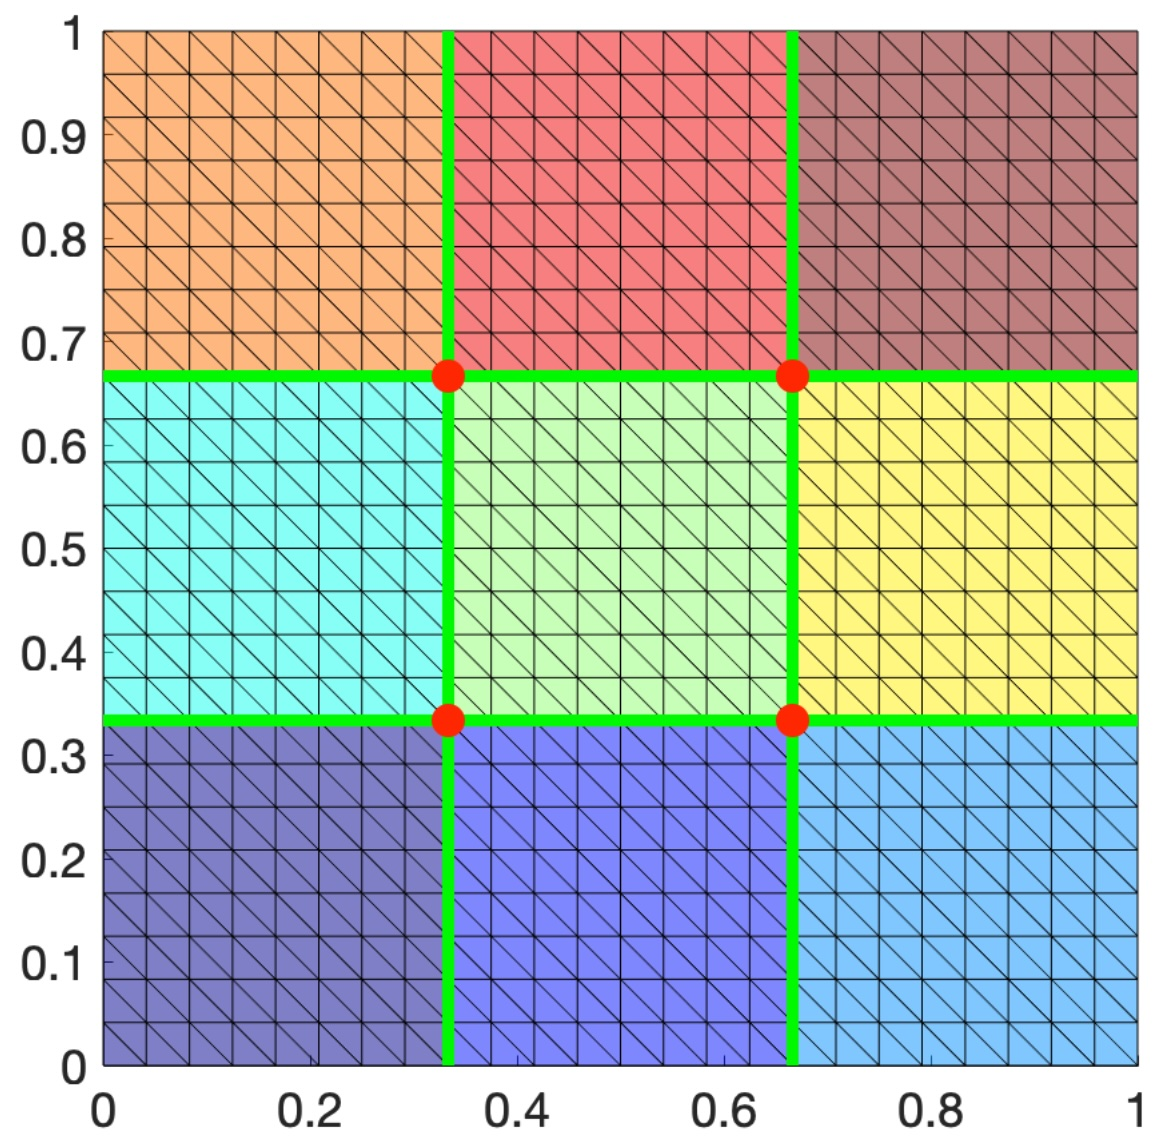
\includegraphics[width=0.5\textwidth]{images/decomposed_domain.jpg}
				\end{figure}
			\end{column}
			\begin{column}{0.49\textwidth}
				\vspace*{-6mm}
				\begin{figure}
					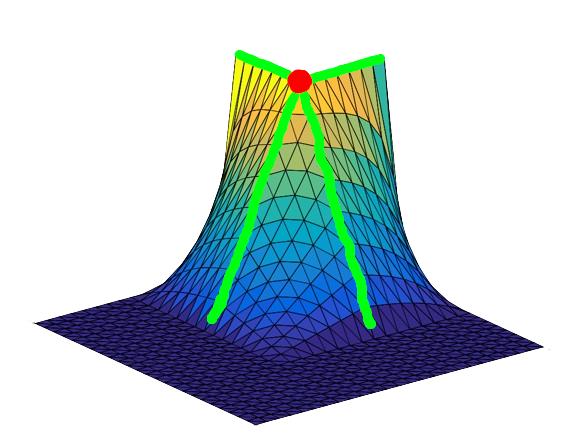
\includegraphics[width=0.6\textwidth]{images/r22.png}
				\end{figure}
			\end{column}
		\end{columns}
	}
	\only<3>{
		Summary:
		\begin{equation*}
			\Phi =
			\begin{pmatrix}
				\Phi_I \\  \Phi_\Gamma
			\end{pmatrix} =
			\begin{pmatrix}
				-A_{II}^{-1}A_{I\Gamma}\Phi_\Gamma \\ \Phi_\Gamma
			\end{pmatrix}
		\end{equation*}
		and
		\begin{equation*}
			P_0 \coloneqq \Phi\text{,}\quad R_0 \coloneqq \Phi^T
		\end{equation*}
	}
\end{frame}

\begin{frame}[noframenumbering]{Nonlinear Schwarz domain decomposition methods}% \footnote{\tiny Cai and Keyes 2002} \footnote{\tiny Dolean, Gander, Cherie, Kwok and Masson 2016}}
	\vspace{-5mm}
	\begin{columns}
		\begin{column}{0.7\textwidth}
      \centering
			\begin{block}{\normalsize Alternative nonlinear problem}
				The discretized nonlinear partial differential equation
				\begin{equation*}
					F(u) = 0,\, F : V\mapsto V
				\end{equation*}
				is reformulated to
				\begin{equation*}
          \mathcal{F}(u) = 0,\, \mathcal{F} : V\mapsto V.
				\end{equation*}
				The new nonlinear function $\mathcal{F}(u)$ is given implicitly by computing local nonlinear corrections $T_i(u),\,i = 1,\dots,N$ on (overlapping) subdomains
			\end{block}
		\end{column}
		\begin{column}{0.3\textwidth}
			\begin{figure}
				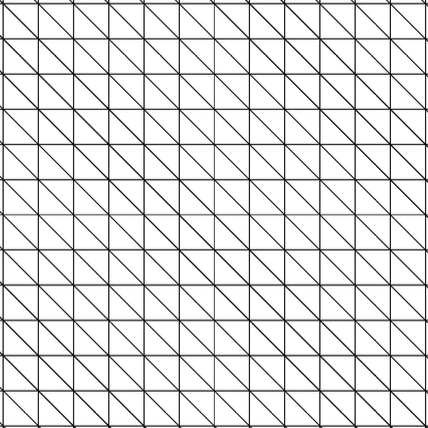
\includegraphics[height=0.4\textwidth,width=0.7\textwidth]{images/DD-mesh-1.png}
				\vspace{-2mm}
				\caption{\tiny Global domain $\Omega$, FE space $V$}
			\end{figure}
			\vspace{-6mm}
			\begin{figure}
				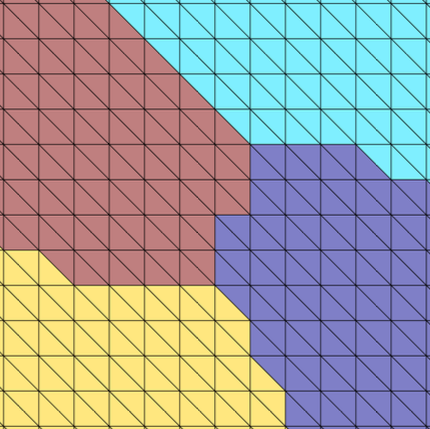
\includegraphics[height=0.4\textwidth,width=0.7\textwidth]{images/DD-mesh-2.png}
				\vspace{-2mm}
				\caption{\tiny Subdomains $\Omega_i$, FE spaces $V(\Omega_i)$}
			\end{figure}
			\vspace{-6mm}
			\begin{figure}
				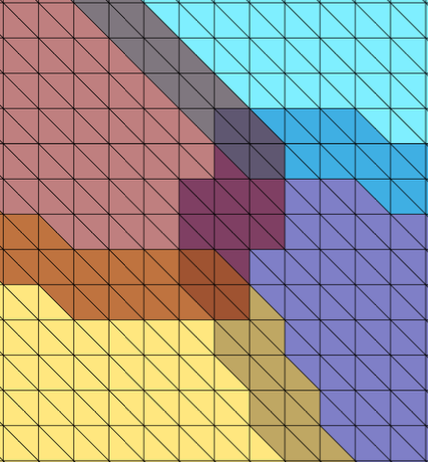
\includegraphics[height=0.4\textwidth,width=0.7\textwidth]{images/DD-mesh-3.png}
				\vspace{-2mm}
				\caption{\tiny Overlapping SDs $\Omega_i'$, FE spaces $V_i$}
			\end{figure}
		\end{column}

	\end{columns}
\end{frame}


\begin{frame}[noframenumbering]{LDC coarse basis functions}
	\begin{figure}
		\centering
		\begin{subfigure}{0.5\textwidth}
			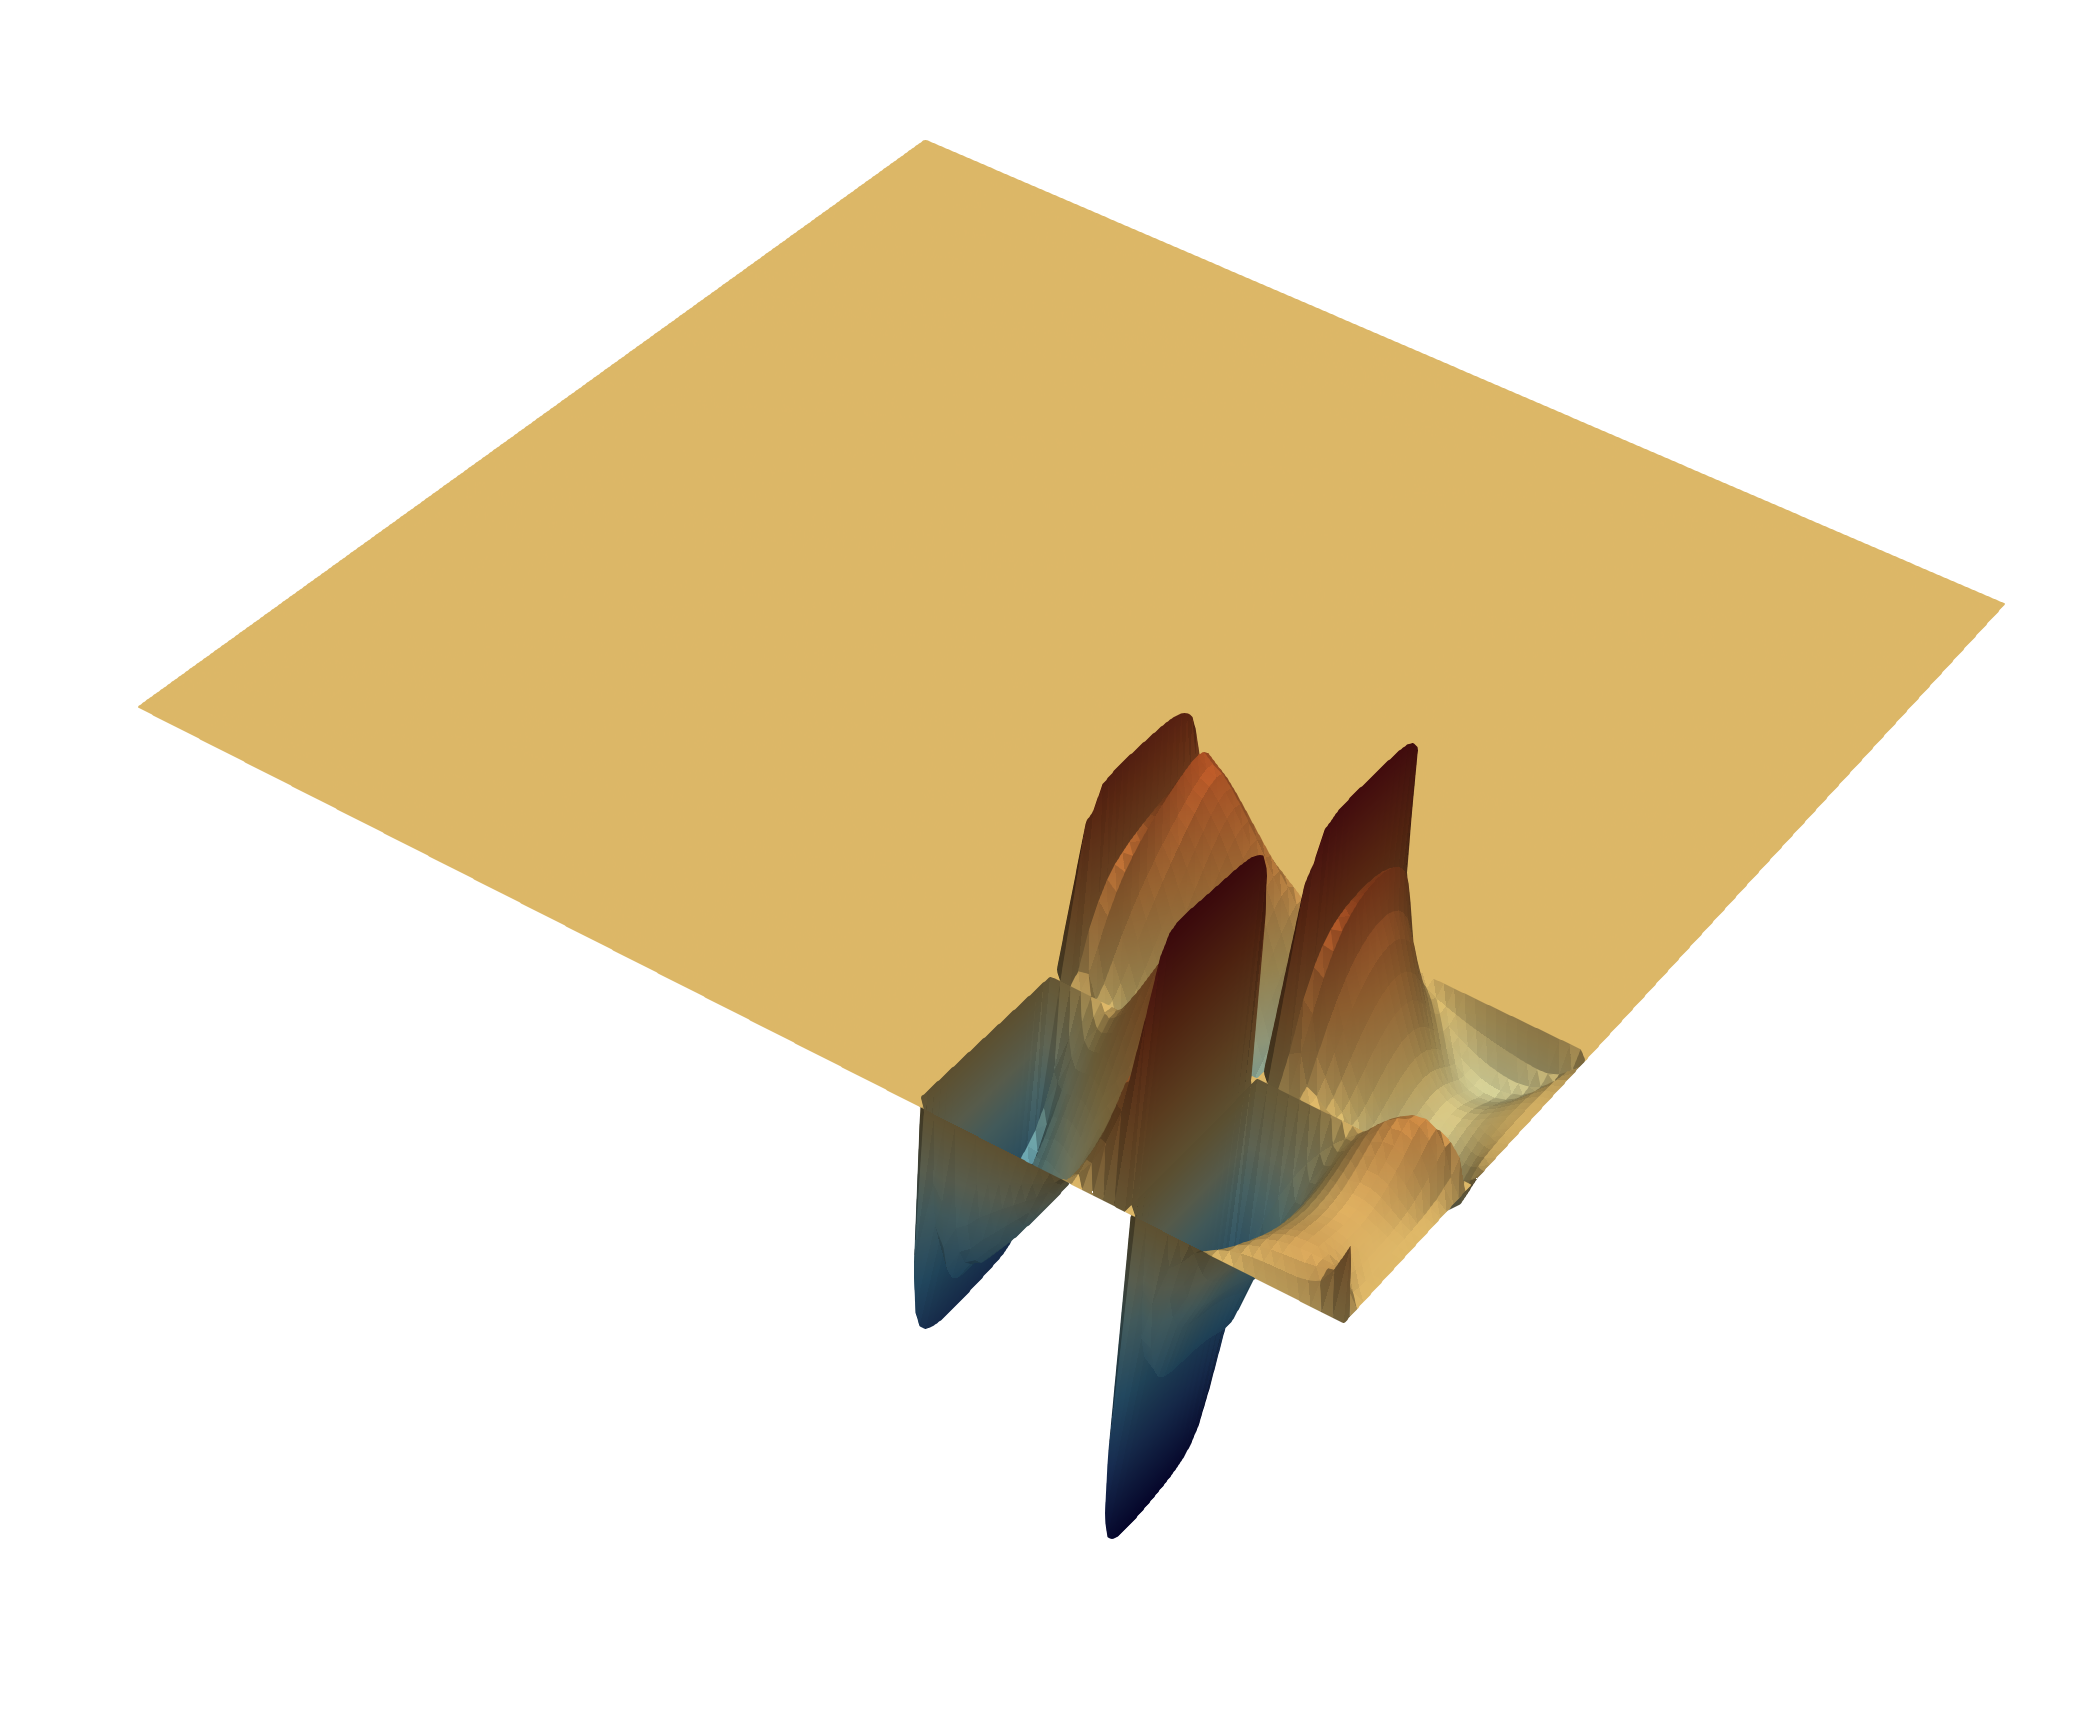
\includegraphics[width=\textwidth]{images/RGDSW-y}
			\caption{RGDSW $y$ component.}
		\end{subfigure}%
		\begin{subfigure}{0.5\textwidth}
			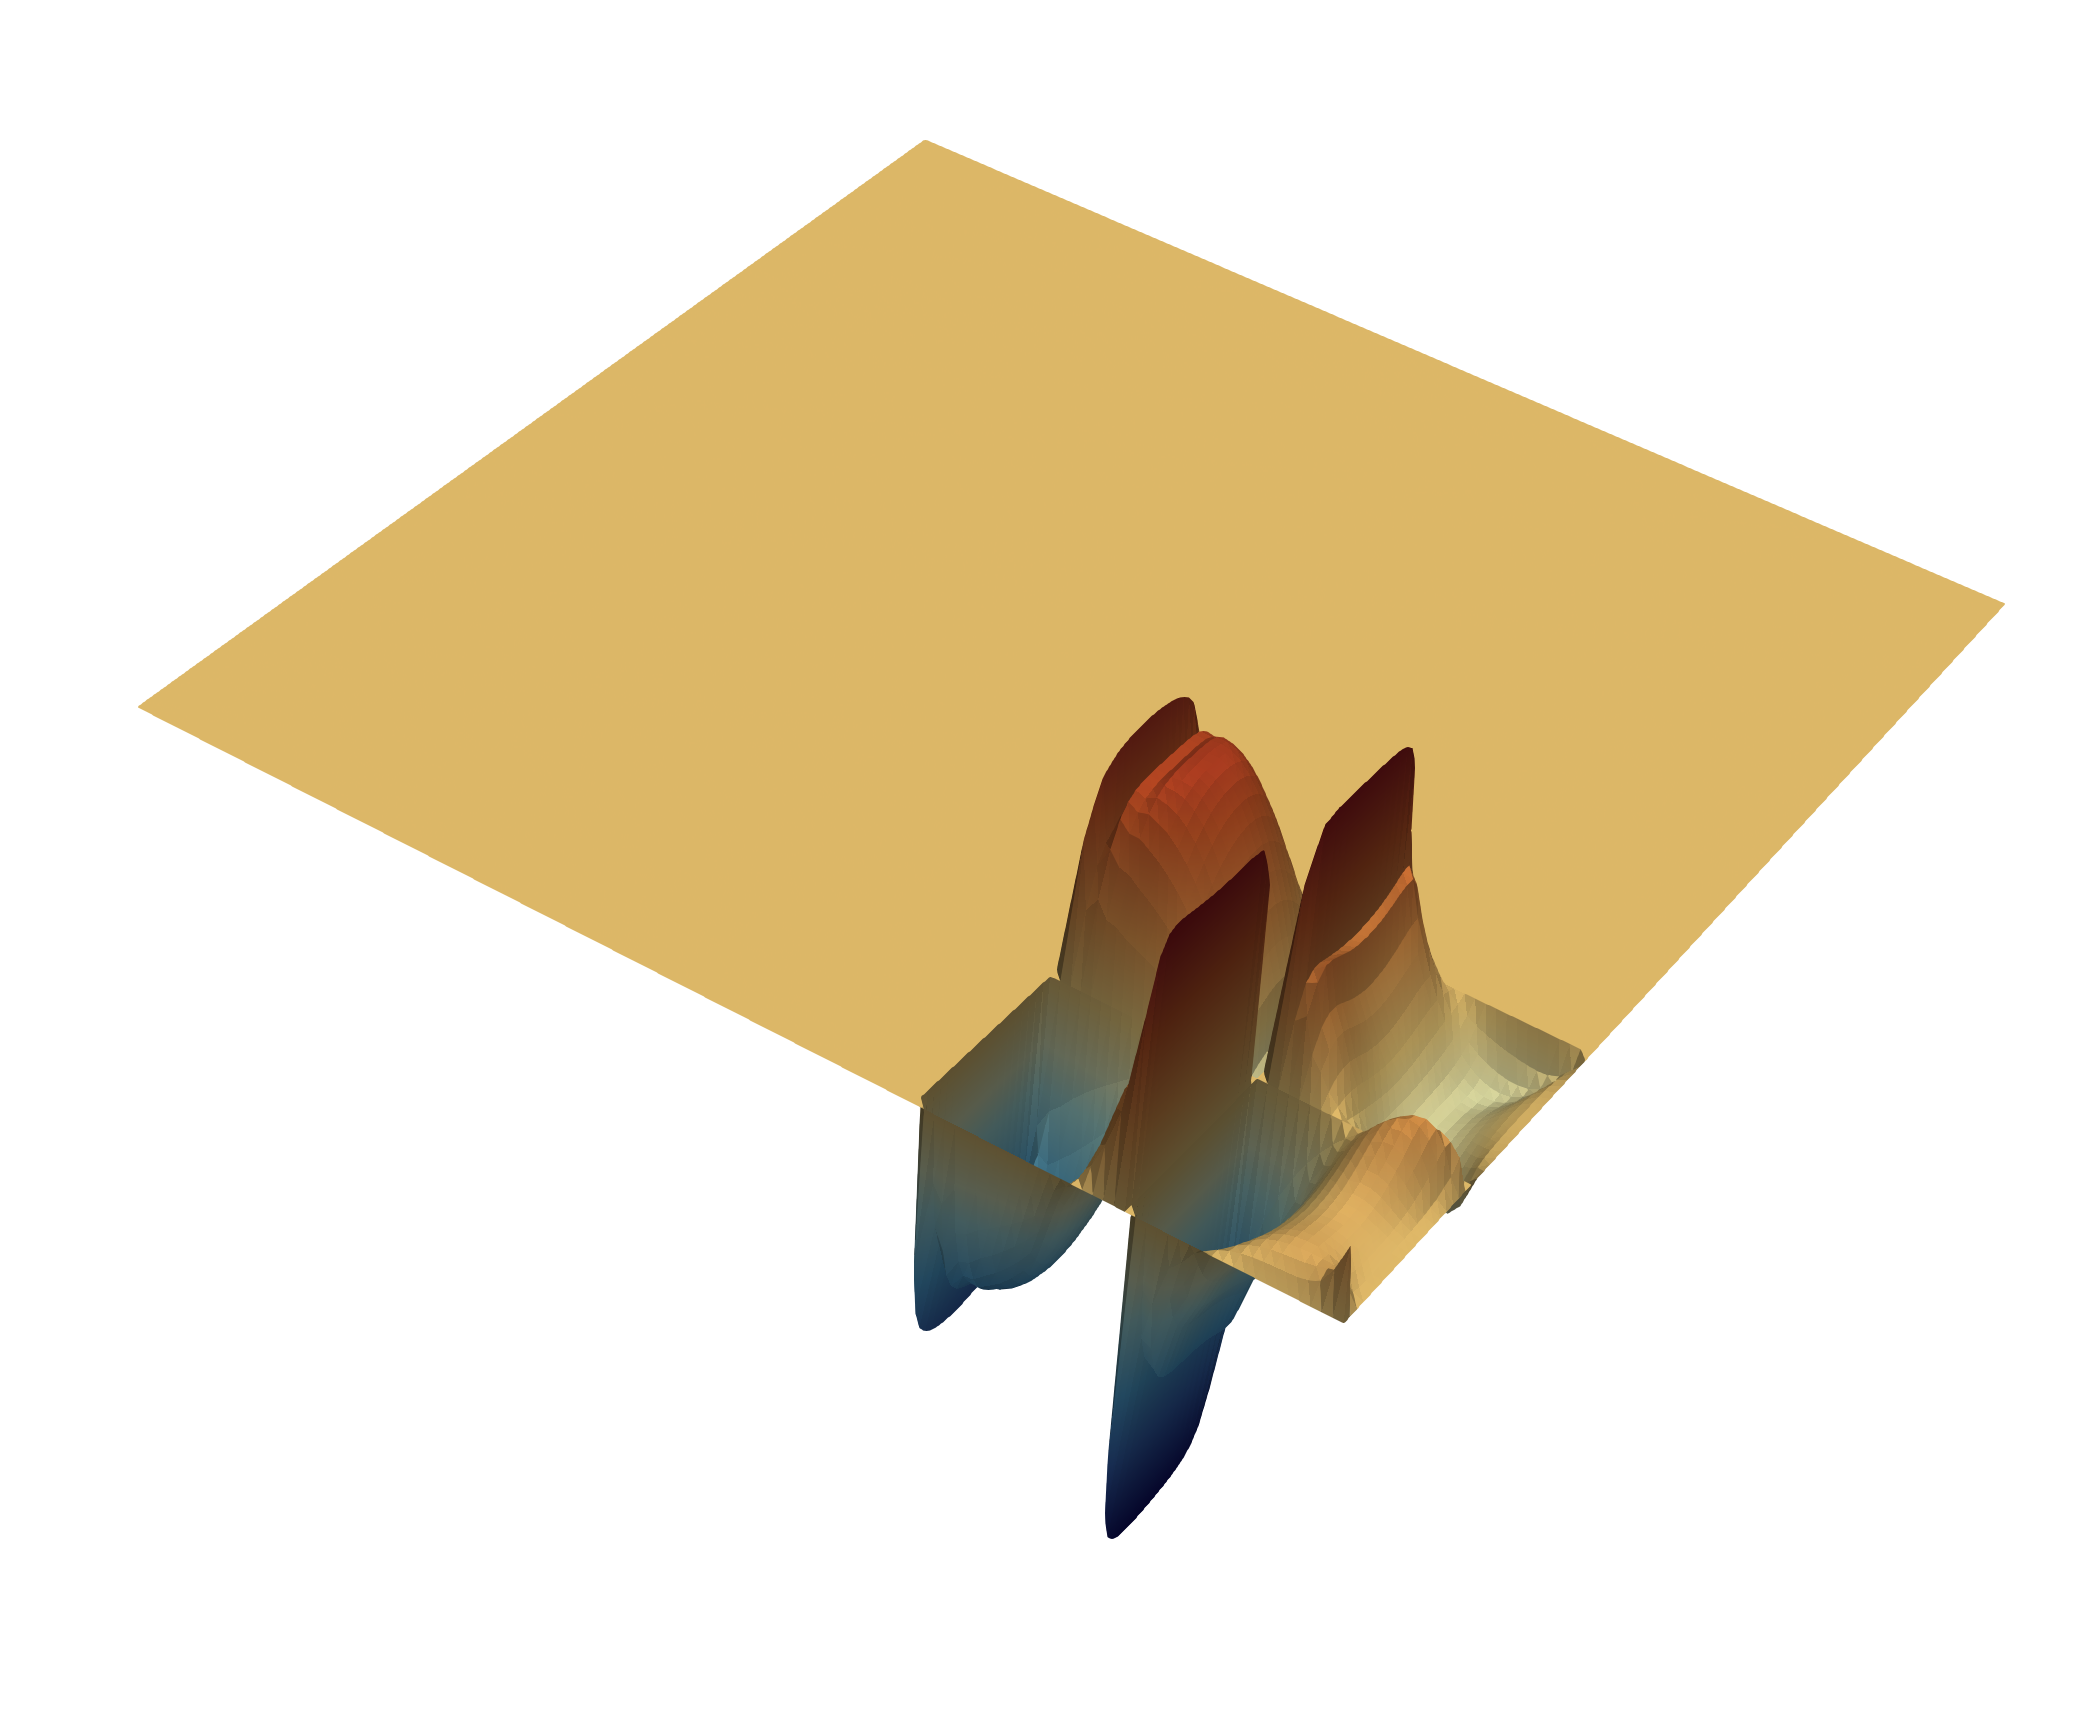
\includegraphics[width=\textwidth]{images/MsFEM-y}
			\caption{MsFEM $y$ component.}
		\end{subfigure}
		\caption{Components of $x$ velocity coarse basis function.}
	\end{figure}
\end{frame}
